\section{Visualización}

\subsection{Visualización de las medidas de la primera práctica}

\begin{figure}[H]
\centering
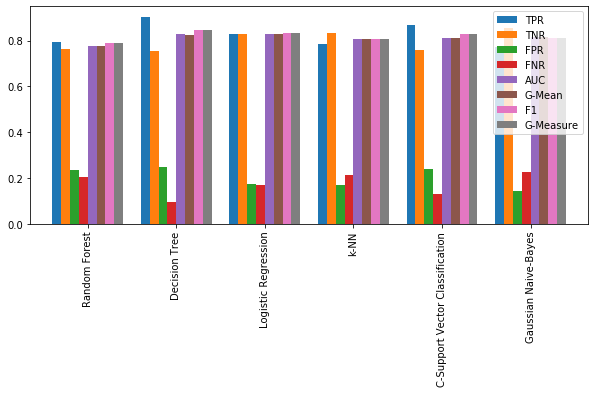
\includegraphics[width=0.8\textwidth]{imagenes/pre-delete.png}
\caption{Medidas obtenidas eliminando valores perdidos}
\end{figure}

\begin{figure}[H]
\centering
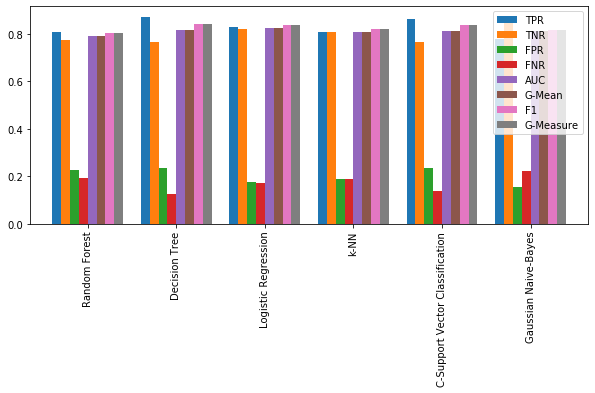
\includegraphics[width=0.8\textwidth]{imagenes/pre-mean.png}
\caption{Medidas obtenidas tratando los valores perdidos usando la media}
\end{figure}

\begin{figure}[H]
\centering
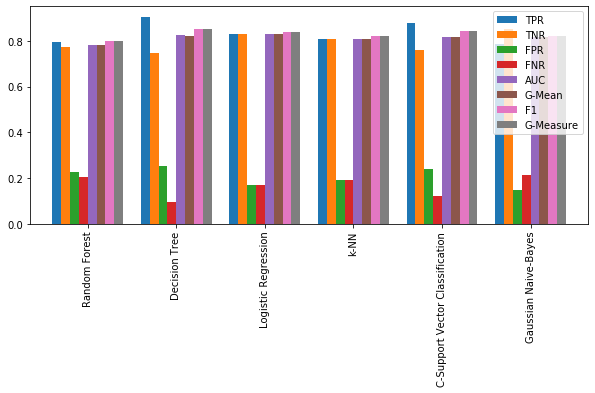
\includegraphics[width=0.8\textwidth]{imagenes/pre-median.png}
\caption{Medidas obtenidas tratando los valores perdidos usando la mediana}
\end{figure}

\begin{figure}[H]
\centering
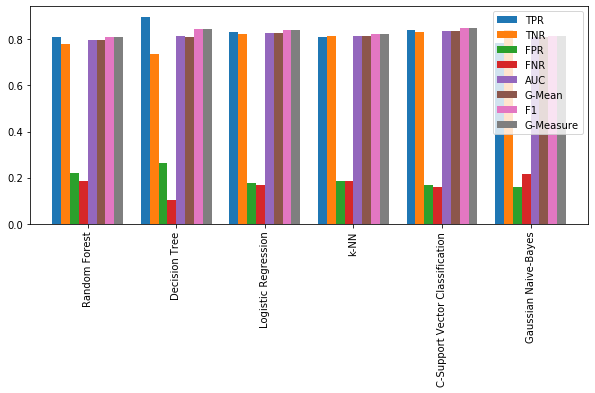
\includegraphics[width=0.8\textwidth]{imagenes/pre-most-freq.png}
\caption{Medidas obtenidas tratando los valores perdidos usando el valor más frecuente}
\end{figure}

\begin{figure}[H]
\centering
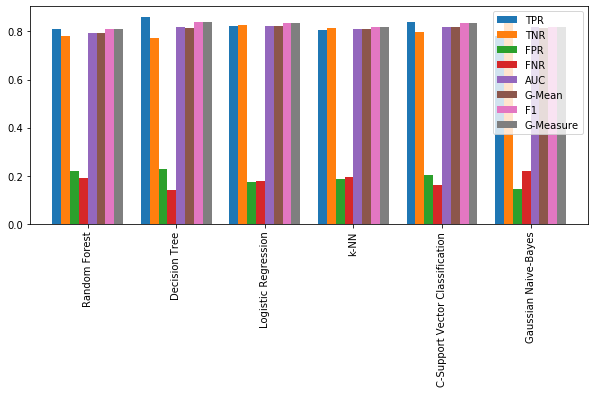
\includegraphics[width=0.8\textwidth]{imagenes/pre-knn11.png}
\caption{Medidas obtenidas tratando los valores perdidos usando k-NN con 11 vecinos}
\end{figure}

\subsection{Curvas ROC}

\begin{figure}[H]
\centering
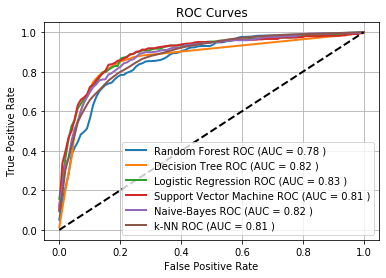
\includegraphics[width=0.8\textwidth]{imagenes/roc_curve.png}
\caption{Curva ROC de los distintos modelos de la primera práctica}
\end{figure}

